\section{The platforms that build system of e-commerce - Overview}
\label{sec:platform_overview}
The platforms that help build a system of e-commerce are exactly systems or portals that facilitate the life of a traded that want to start your own online business.
\newline
The process of setting up an online store with such systems is very fast and efficient, because essential information is easy to fit. The next moment is the choice of the graphical presentation of the store where the trader can choose from many themes and templates available.
These systems handle transparently different services that help create the store such as: the domain, payment management, organizing inventory, shipping and tracking of shipments, invoice management, etc..
\newline
The advantages and disadvantages of these platforms are mainly linked to the flexibility of the system itself. In fact, a platform for e-commerce-rich services, has more chance of being used by a growing number of major traded.
\newline
Obviously, a generic platform so can not meet the needs of every type of merchant because the platform has the purpose of facilitating the realization of a system of e-commerce in a more simple possibilie. Therefore it is difficult to meet the needs of each merchant from any kind of detail. Ease of use is another key point that leads to the platform to be chosen by dealers.
\newline
The platform of e-commerce are the most famous Shopify, BigCommerce, etc..
\subsection{Shopify}
Shopify is a Canadian commerce company headquartered in Ottawa, Ontario that develops computer software for online stores and retail point-of-sale systems.
\newline
Shopify was founded in 2004, and was initially based on earlier software written by its founders for their online snowboard store. The company reports that it has 200,000 merchants using its platform, with total gross merchandise volume exceeding \$10 billion.
\begin{figure}[htb]
 \centering
 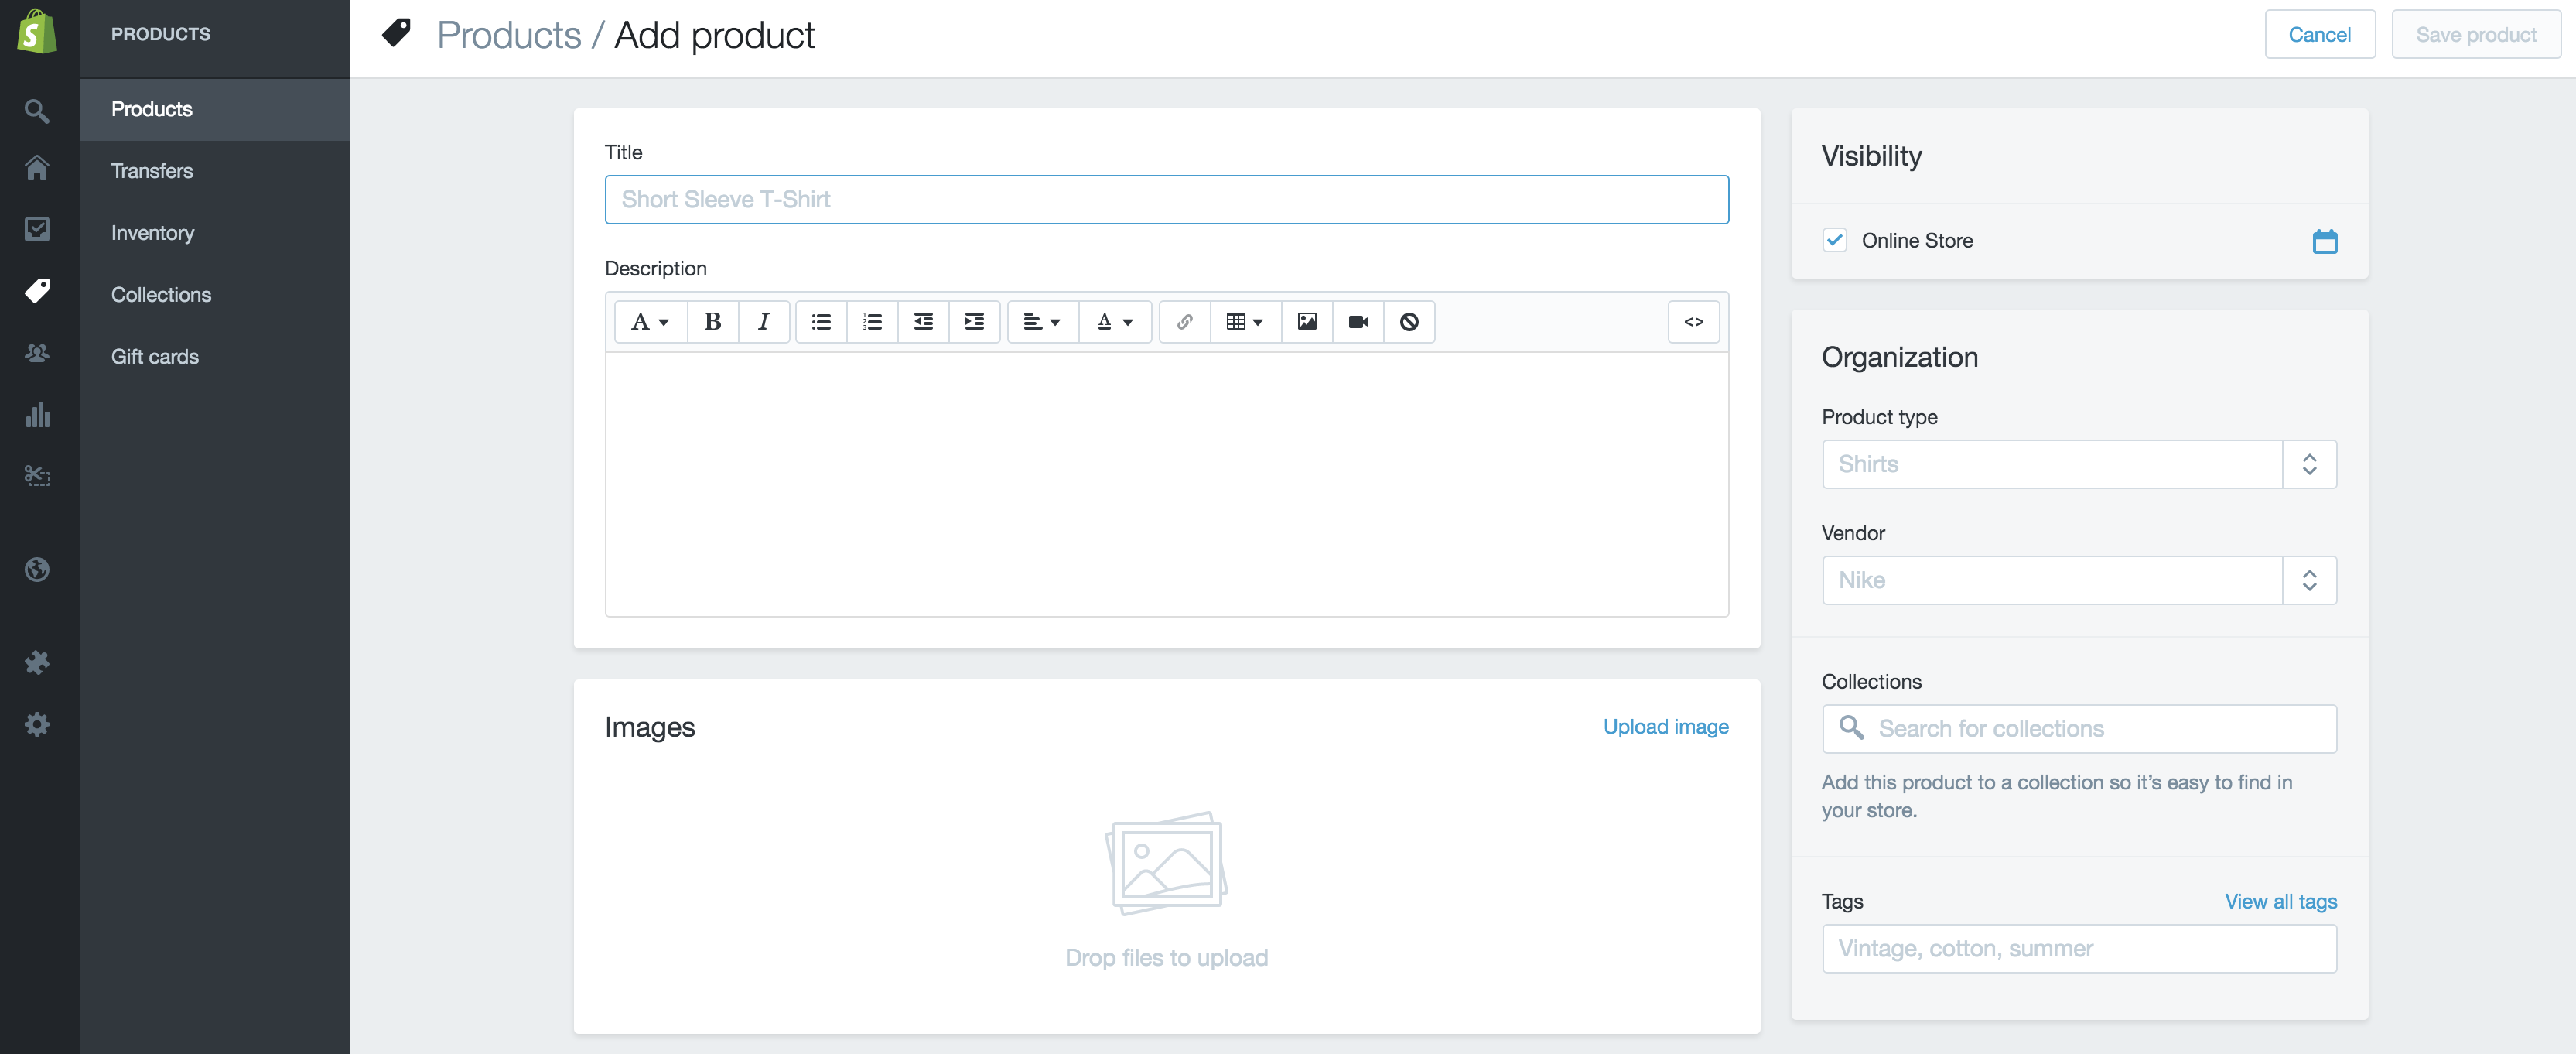
\includegraphics[width=1.0\linewidth]{images/chapter1/ex-shopify.png}\hfill
 \caption[Shopify Dashboard]{Shopify Dashboard}
 \label{fig:shopify_dashboard}
\end{figure}
Shopify was founded in 2004 by Tobias Lütke, Daniel Weinand, and Scott Lake after attempting to open Snowdevil, an online store for snowboarding equipment. Unsatisfied with the existing e-commerce products on the market, Lütke, a programmer by trade, decided to build his own.
Lütke used the open source web application framework. Ruby on Rails to build Snowdevil's online store, and launched it after two months of development The Snowdevil founders launched the platform as Shopify in June 2006.
In September 2015, Amazon announced it would be closing its Amazon Webstore service for merchants, and had selected Shopify as the preferred migration provider. Shopify's shares jumped more than 20\% upon the news.

\subsection{Bigcommerce}
Bigcommerce is a privately held technology company that develops e-commerce software for businesses. The company was founded in 2009 and has 370 employees with headquarters in Austin, Texas and additional offices in San Francisco, California and Sydney, Australia.
The company reports that \$5 billion in total sales have been processed by the Bigcommerce platform.
\begin{figure}[htb]
 \centering
 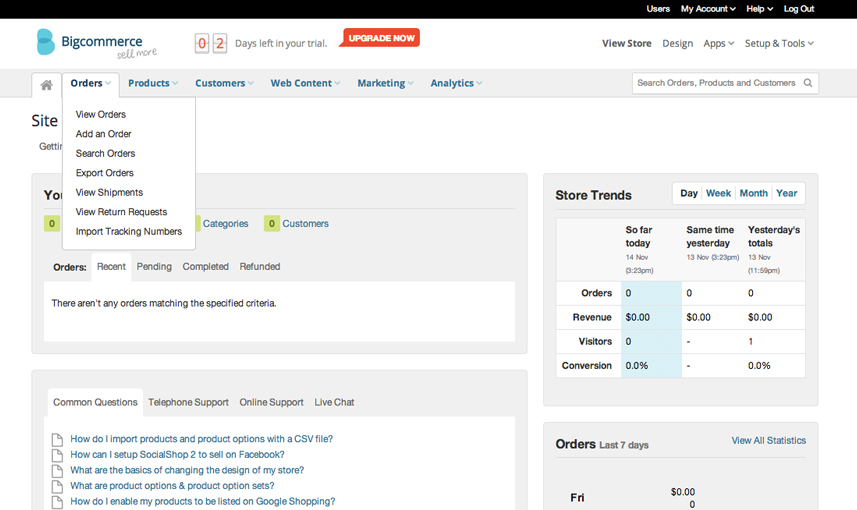
\includegraphics[width=1.0\linewidth]{images/chapter1/ex-bigcommerce.jpg}\hfill
 \caption[Bigcommerce Dashboard]{Bigcommerce Dashboard}
 \label{fig:bigcommerce_dashboard}
\end{figure}
Bigcommerce was founded in 2009 by Australians Eddie Machaalani and Mitchell Harper following a chance meeting in an online chatroom in 2003. In August 2009, the two relaunched a hosted version of Interspire Shopping Cart called “BigCommerce” and opened its first U.S. office.
\newline
Bigcommerce was 100\% bootstrapped until July 31, 2011, when it closed \$15 million in Series A funding from General Catalyst Partners. At the time, the company announced its client count had grown 680\% year over year.
\newline
In January 2012, Bigcommerce launched a \$2 million integration fund for developers, which was used to fund 31 applications in the Bigcommerce App Marketplace. The company subsequently received \$20 million in Series B financing in September 2012, led by General Catalyst Partners and Floodgate Fund.